\documentclass{standalone}
\usepackage{tikz}
\usetikzlibrary{patterns, positioning}


\begin{document}
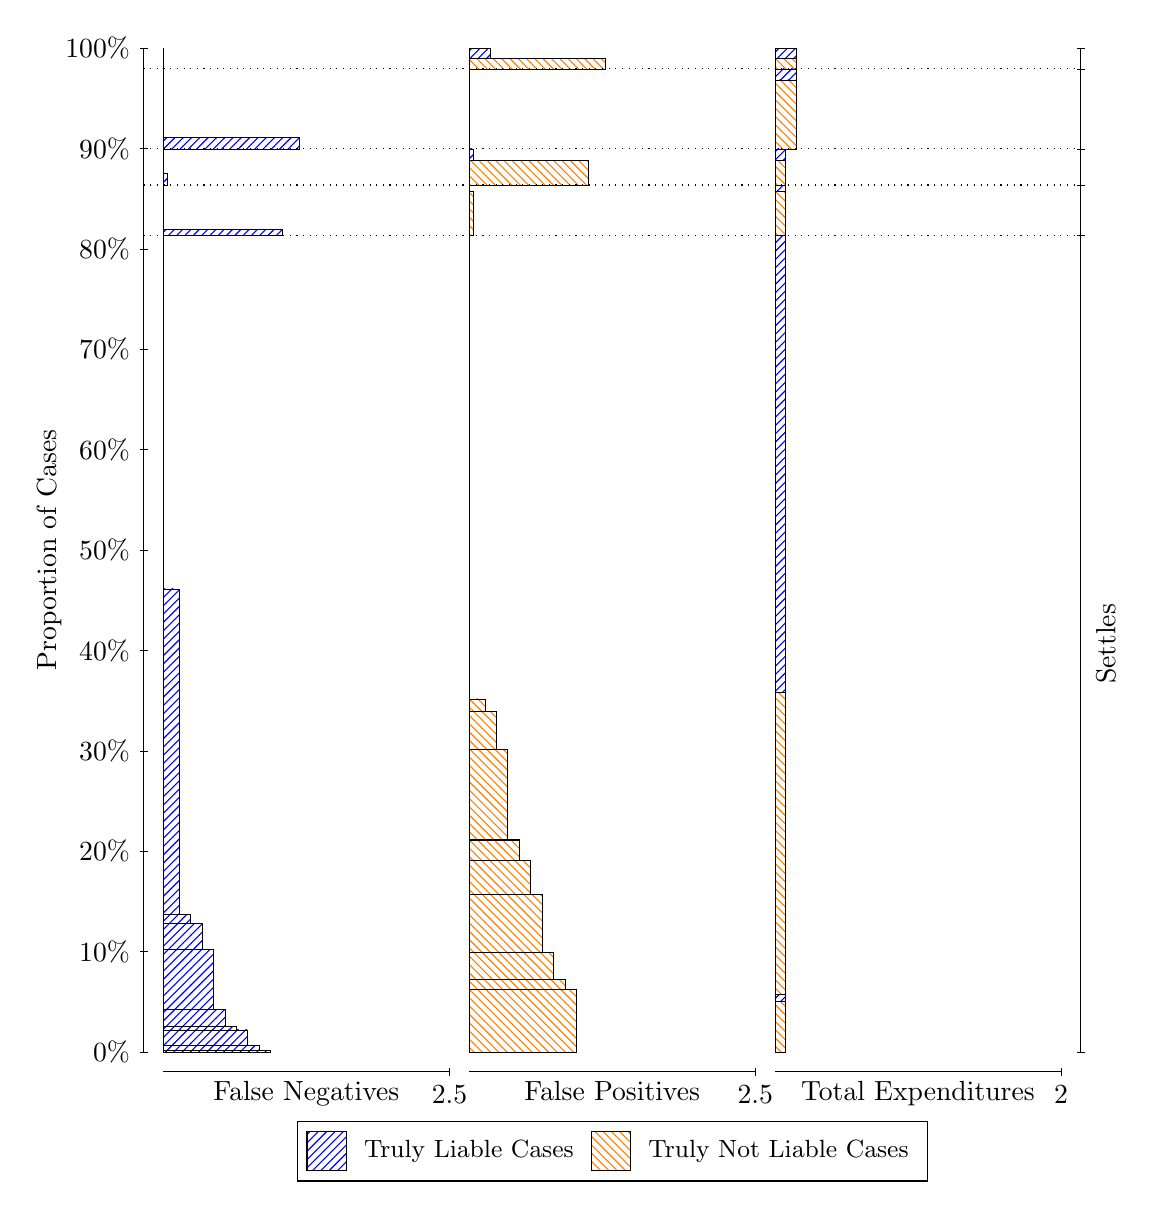
\begin{tikzpicture}
\draw[black, very thin] (1.5,1.75) -- (1.5,14.5);
\node[rotate=90, text=black, anchor=center] at (0.3, 8.125) {Proportion of Cases};
\draw[black, very thin] (1.45,1.75) -- (1.55,1.75);
\node[text=black, anchor=east] at (1.45, 1.75) {0\%};
\draw[black, very thin] (1.45,3.025) -- (1.55,3.025);
\node[text=black, anchor=east] at (1.45, 3.025) {10\%};
\draw[black, very thin] (1.45,4.3) -- (1.55,4.3);
\node[text=black, anchor=east] at (1.45, 4.3) {20\%};
\draw[black, very thin] (1.45,5.575) -- (1.55,5.575);
\node[text=black, anchor=east] at (1.45, 5.575) {30\%};
\draw[black, very thin] (1.45,6.85) -- (1.55,6.85);
\node[text=black, anchor=east] at (1.45, 6.85) {40\%};
\draw[black, very thin] (1.45,8.125) -- (1.55,8.125);
\node[text=black, anchor=east] at (1.45, 8.125) {50\%};
\draw[black, very thin] (1.45,9.4) -- (1.55,9.4);
\node[text=black, anchor=east] at (1.45, 9.4) {60\%};
\draw[black, very thin] (1.45,10.675) -- (1.55,10.675);
\node[text=black, anchor=east] at (1.45, 10.675) {70\%};
\draw[black, very thin] (1.45,11.95) -- (1.55,11.95);
\node[text=black, anchor=east] at (1.45, 11.95) {80\%};
\draw[black, very thin] (1.45,13.225) -- (1.55,13.225);
\node[text=black, anchor=east] at (1.45, 13.225) {90\%};
\draw[black, very thin] (1.45,14.5) -- (1.55,14.5);
\node[text=black, anchor=east] at (1.45, 14.5) {100\%};

\draw[black, very thin] (13.4,1.75) -- (13.4,14.5);
\draw[black, very thin] (13.35,1.75) -- (13.45,1.75);
\node[anchor=west] at (13.35, 1.75) {};
\draw[black, very thin] (13.35,12.116) -- (13.45,12.116);
\node[anchor=west] at (13.35, 12.116) {};
\draw[black, very thin] (13.35,12.76) -- (13.45,12.76);
\node[anchor=west] at (13.35, 12.76) {};
\draw[black, very thin] (13.35,13.22) -- (13.45,13.22);
\node[anchor=west] at (13.35, 13.22) {};
\draw[black, very thin] (13.35,14.235) -- (13.45,14.235);
\node[anchor=west] at (13.35, 14.235) {};
\draw[black, very thin] (13.35,14.5) -- (13.45,14.5);
\node[anchor=west] at (13.35, 14.5) {};

\draw[black, very thin, pattern color=blue, pattern=north east lines] (1.75,1.75) rectangle (3.1125,1.7698);
\draw[black, very thin, pattern color=blue, pattern=north east lines] (1.75,1.7698) rectangle (2.9672,1.8362);
\draw[black, very thin, pattern color=blue, pattern=north east lines] (1.75,1.8362) rectangle (2.8218,2.0294);
\draw[black, very thin, pattern color=blue, pattern=north east lines] (1.75,2.0294) rectangle (2.6765,2.0725);
\draw[black, very thin, pattern color=blue, pattern=north east lines] (1.75,2.0725) rectangle (2.5312,2.2876);
\draw[black, very thin, pattern color=blue, pattern=north east lines] (1.75,2.2876) rectangle (2.3858,3.0563);
\draw[black, very thin, pattern color=blue, pattern=north east lines] (1.75,3.0563) rectangle (2.2405,3.3831);
\draw[black, very thin, pattern color=blue, pattern=north east lines] (1.75,3.3831) rectangle (2.0952,3.4933);
\draw[black, very thin, pattern color=blue, pattern=north east lines] (1.75,3.4933) rectangle (1.9498,7.6305);
\draw[black, very thin, pattern color=orange, pattern=north west lines] (1.75,7.6305) rectangle (1.75,12.116);
\draw[black, very thin, pattern color=blue, pattern=north east lines] (1.75,12.116) rectangle (3.2578,12.197);
\draw[black, very thin, pattern color=orange, pattern=north west lines] (1.75,12.197) rectangle (1.75,12.76);
\draw[black, very thin, pattern color=blue, pattern=north east lines] (1.75,12.76) rectangle (1.8045,12.905);
\draw[black, very thin, pattern color=orange, pattern=north west lines] (1.75,12.905) rectangle (1.75,13.22);
\draw[black, very thin, pattern color=blue, pattern=north east lines] (1.75,13.22) rectangle (3.4758,13.362);
\draw[black, very thin, pattern color=orange, pattern=north west lines] (1.75,13.362) rectangle (1.75,14.235);
\draw[black, very thin, pattern color=orange, pattern=north west lines] (1.75,14.235) rectangle (1.75,14.373);
\draw[black, very thin, pattern color=blue, pattern=north east lines] (1.75,14.373) rectangle (1.75,14.5);
\draw[black, very thin, pattern color=orange, pattern=north west lines] (5.6333,1.75) rectangle (6.9958,2.5455);
\draw[black, very thin, pattern color=orange, pattern=north west lines] (5.6333,2.5455) rectangle (6.8505,2.667);
\draw[black, very thin, pattern color=orange, pattern=north west lines] (5.6333,2.667) rectangle (6.7052,3.0131);
\draw[black, very thin, pattern color=orange, pattern=north west lines] (5.6333,3.0131) rectangle (6.5598,3.7531);
\draw[black, very thin, pattern color=orange, pattern=north west lines] (5.6333,3.7531) rectangle (6.4145,4.1865);
\draw[black, very thin, pattern color=orange, pattern=north west lines] (5.6333,4.1865) rectangle (6.2692,4.4372);
\draw[black, very thin, pattern color=orange, pattern=north west lines] (5.6333,4.4372) rectangle (6.2692,4.4522);
\draw[black, very thin, pattern color=orange, pattern=north west lines] (5.6333,4.4522) rectangle (6.1238,5.5909);
\draw[black, very thin, pattern color=orange, pattern=north west lines] (5.6333,5.5909) rectangle (5.9785,6.0791);
\draw[black, very thin, pattern color=orange, pattern=north west lines] (5.6333,6.0791) rectangle (5.8332,6.2353);
\draw[black, very thin, pattern color=blue, pattern=north east lines] (5.6333,6.2353) rectangle (5.6333,12.116);
\draw[black, very thin, pattern color=orange, pattern=north west lines] (5.6333,12.116) rectangle (5.6878,12.679);
\draw[black, very thin, pattern color=blue, pattern=north east lines] (5.6333,12.679) rectangle (5.6333,12.76);
\draw[black, very thin, pattern color=orange, pattern=north west lines] (5.6333,12.76) rectangle (7.1412,13.075);
\draw[black, very thin, pattern color=blue, pattern=north east lines] (5.6333,13.075) rectangle (5.6878,13.22);
\draw[black, very thin, pattern color=orange, pattern=north west lines] (5.6333,13.22) rectangle (5.6333,14.094);
\draw[black, very thin, pattern color=blue, pattern=north east lines] (5.6333,14.094) rectangle (5.6333,14.235);
\draw[black, very thin, pattern color=orange, pattern=north west lines] (5.6333,14.235) rectangle (7.3592,14.373);
\draw[black, very thin, pattern color=blue, pattern=north east lines] (5.6333,14.373) rectangle (5.9058,14.5);
\draw[black, very thin, pattern color=orange, pattern=north west lines] (9.5167,1.75) rectangle (9.6529,2.3944);
\draw[black, very thin, pattern color=blue, pattern=north east lines] (9.5167,2.3944) rectangle (9.6529,2.4806);
\draw[black, very thin, pattern color=orange, pattern=north west lines] (9.5167,2.4806) rectangle (9.6529,6.3215);
\draw[black, very thin, pattern color=blue, pattern=north east lines] (9.5167,6.3215) rectangle (9.6529,12.116);
\draw[black, very thin, pattern color=orange, pattern=north west lines] (9.5167,12.116) rectangle (9.6529,12.679);
\draw[black, very thin, pattern color=blue, pattern=north east lines] (9.5167,12.679) rectangle (9.6529,12.76);
\draw[black, very thin, pattern color=orange, pattern=north west lines] (9.5167,12.76) rectangle (9.6529,13.075);
\draw[black, very thin, pattern color=blue, pattern=north east lines] (9.5167,13.075) rectangle (9.6529,13.22);
\draw[black, very thin, pattern color=orange, pattern=north west lines] (9.5167,13.22) rectangle (9.7892,14.094);
\draw[black, very thin, pattern color=blue, pattern=north east lines] (9.5167,14.094) rectangle (9.7892,14.235);
\draw[black, very thin, pattern color=orange, pattern=north west lines] (9.5167,14.235) rectangle (9.7892,14.373);
\draw[black, very thin, pattern color=blue, pattern=north east lines] (9.5167,14.373) rectangle (9.7892,14.5);
\draw[black, dotted] (1.5,12.116) -- (13.4,12.116);
\draw[black, dotted] (1.5,12.76) -- (13.4,12.76);
\draw[black, dotted] (1.5,13.22) -- (13.4,13.22);
\draw[black, dotted] (1.5,14.235) -- (13.4,14.235);
\draw[black, very thin] (1.75,1.5) -- (5.3833,1.5);
\node[text=black, anchor=north] at (3.5667, 1.5) {False Negatives};
\draw[black, very thin] (5.3833,1.45) -- (5.3833,1.55);
\node[text=black, anchor=north] at (5.3833, 1.45) {2.5};

\draw[black, very thin] (5.6333,1.5) -- (9.2667,1.5);
\node[text=black, anchor=north] at (7.45, 1.5) {False Positives};
\draw[black, very thin] (9.2667,1.45) -- (9.2667,1.55);
\node[text=black, anchor=north] at (9.2667, 1.45) {2.5};

\draw[black, very thin] (9.5167,1.5) -- (13.15,1.5);
\node[text=black, anchor=north] at (11.333, 1.5) {Total Expenditures};
\draw[black, very thin] (13.15,1.45) -- (13.15,1.55);
\node[text=black, anchor=north] at (13.15, 1.45) {2};

\node[text=black, centered, rotate=90] at (13.72, 6.9329) {Settles};





\draw (7.449999999999999,1.5) node[draw=none] (baseCoordinate) {};
\begin{scope}[align=center]
        \matrix[scale=0.5, draw=black, below=0.5cm of baseCoordinate, nodes={draw}, column sep=0.1cm]{
            \node[rectangle, draw, minimum width=0.5cm, minimum height=0.5cm, pattern color=blue, pattern=north east lines] {}; &
            \node[draw=none, font=\small, text=black] (B) {Truly Liable Cases}; &
            \node[rectangle, draw, minimum width=0.5cm, minimum height=0.5cm, pattern color=orange, pattern=north west lines] {}; &
            \node[draw=none, font=\small, text=black] (B) {Truly Not Liable Cases}; \\
            };
\end{scope}

\end{tikzpicture}
\end{document}